\chapter{Evaluation und Validation}
\label{ch:evaluation}

% Auswertung und Interpretation der Ergebnisse. Nachweis, dass die Ziele erreicht wurden, oder
% warum welche nicht erreicht wurden.

Quantitative Auswertung

\section{Validation der Testumgebung}

Um Aussagen machen zu können über das Testnetzwerk muss erst sichergestellt werden, dass die Messwerte Sinn ergeben.
Deshalb wurden erste Tests durchgeführt, um zu prüfen, ob die Testumgebung auch richtig funktioniert.

Diese Messungen bieten auch eine Basis und einen Referenzpunkt für die weiteren Messungen.

\subsection{Wiederholbarkeit von Messungen}

Als Teil dieser Messung wird erst ein Netzwerk mit 8 Knoten getestet und die Latenz von 1000 Nachrichten gemessen.
Alle Knoten haben in diesem Test keine Bandbreitenbeschränkung.
Eine Nachricht wird hier jeweils von einem zufälligen Knoten an einen anderen zufälligen Knoten versendet.
Die Konfigurierte Nachrichtengrösse wurde jeweils auf 64kB festgelegt.
Die Messung wird so festgehalten.
Anschliessend wird derselbe Test noch einmal gestartet, wobei das Testnetzwerk jedoch aber neu erstellt wird.

Grundsätzlich wird hier erwartet, dass die Messungen vergleichbar sind und ähnliche Resultate liefern.

Somit kann ausgesagt werden das die Messungen so gut wie möglich reproduzierbar sind \seereq{TREP}.


\subsection{Gleichbleibende Latenz bei Skalierung des Netzwerks}

Um sicherzustellen, dass kein Fehler beispielsweise im implementieren Testnetzwerk oder gar in der i2pd-Software aufzufinden ist, wird diese Messung zu Validierungszwecken durchgeführt.

Alle Knoten haben in diesem Test keine Bandbreitenbeschränkung.
Eine Nachricht wird hier jeweils von einem zufälligen Knoten an einen anderen zufälligen Knoten versendet.
Die konfigurierte Nachrichtengrösse wurde jeweils auf 64kB festgelegt.
Die Messung wird so festgehalten.

Anschliessend wird die gleiche Messung noch einmal gestartet.
Jedoch wird die Anzahl Knoten im Testnetzwerk jeweils verdoppelt.

Es wird angenommen, dass sich die Latenz der Nachrichten im Netzwerk nicht hier verändert.
Dies mag auf den ersten Blick der Hypothese wiedersprechen, jedoch gilt es zu beachten, dass hier alle Knoten dieselbe Bandbreitenbeschränkung haben.
%TODO: ref hypothese

\begin{figure*}[htp]
  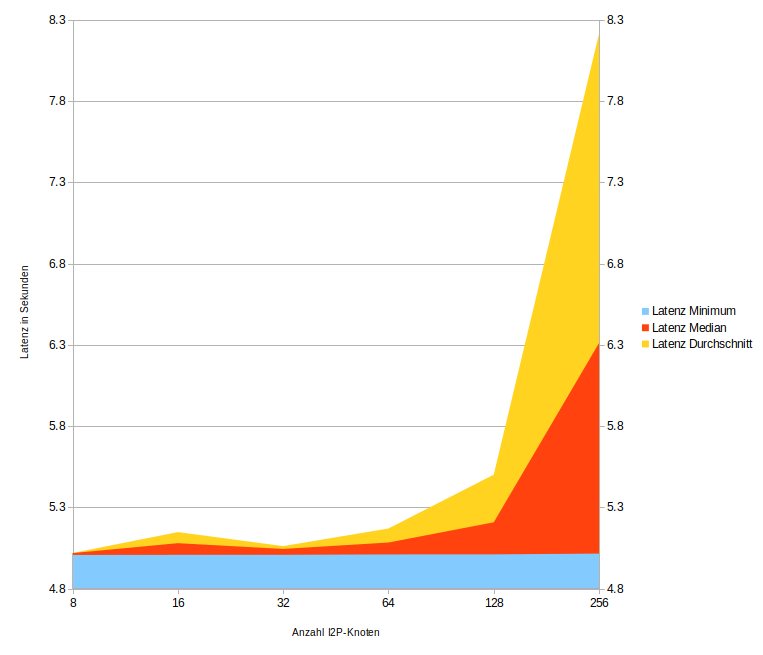
\includegraphics[width=1.1\textwidth]{img/auswertung-latenz.png}
  \caption{Veränderung der Latenz}\label{fig:auswertung-latenz}
\end{figure*}


\subsection{Verhalten der Latenz abhängig von der Nachrichtengrösse}

Bei dieser Messung wurden in einem Testnetzwerk bestehend aus 64 Knoten verschieden grosse Nachrichten versandt.

\section{Vergleich mit Anforderungen}
\label{sec:VergleichAnforderungen}
TODO Vergleich mit Anforderungen Soll<->Ist

\seereq{TNET}

E.g. Diese und diese Anforderungen wurden erreicht, indem dies und das gemacht wurde.
Die Optionalen Anforderungne XY wurden nicht erreicht.

\section{Technische Aspekte}
TODO: Evaluation der verwendeten Hilfsmittel

\subsection{Architektur}

Mit der Umstellung auf die auf \lstinline|docker-compose| basierende Lösung sind leider 


Dementsprechend kann mit diesem Ansatz nicht auf beliebig viele Knoten skaliert werden, da schlussendlich vertikal skaliert wird und dieser Ansatz somit durch existierende Hardware limitiert ist.
Denn die Docker-Container werden mit \lstinline|docker-compose| so nur auf einem einzelnen Rechner erstellt und es können nicht mehrere Testnetzwerke miteinander verbunden werden.

\section{Vorgehen}

TODO :Evaluation der verwendeten Arbeitsprozesse

* Meeting-Notizen (overhead)
